\documentclass{standalone}

\usepackage{tikz}
\usetikzlibrary{patterns}
\usetikzlibrary{arrows.meta}

\begin{document}

	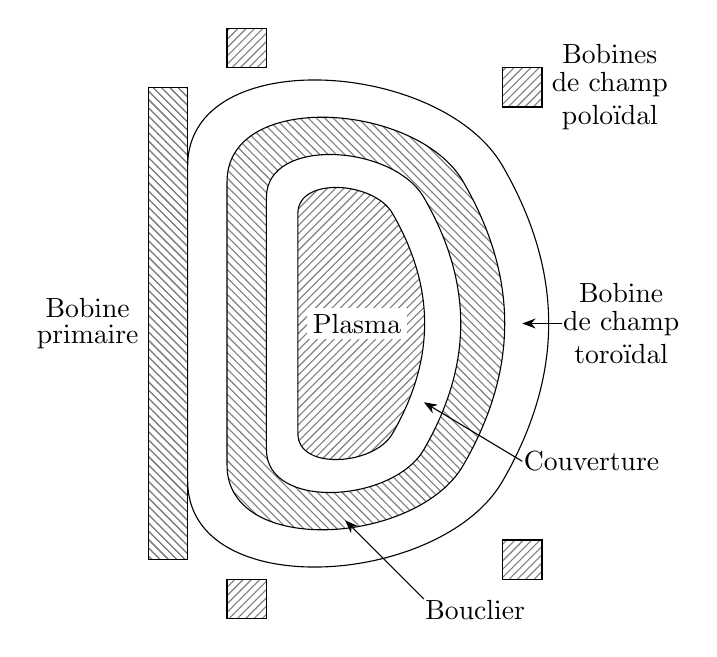
\begin{tikzpicture}
	
		\def\sizex{2}
		\def\sizey{2}
		
		\fill[pattern=north west lines, pattern color=gray]
			(-\sizex, 1.5*\sizey) -- (-\sizex-\sizex/4, 1.5*\sizey) -- (-\sizex-\sizex/4, -1.5*\sizey) -- (-\sizex, -1.5*\sizey) -- cycle;
		\draw[pattern=north west lines, pattern color=gray]
			(-\sizex, 1.5*\sizey) -- (-\sizex-\sizex/4, 1.5*\sizey) -- (-\sizex-\sizex/4, -1.5*\sizey) -- (-\sizex, -1.5*\sizey) -- cycle;
			\node[anchor=east, align=center] at (-\sizex-\sizex/4, 0)  {\shortstack{Bobine\\ primaire}};
			
		\def\anglein{120}
		\def\angleout{60}
		\def\anfleinner{80}
		\fill[white]
			(-\sizex, -\sizey) -- (-\sizex, \sizey) to [out=\anfleinner, in=\anglein] (\sizex, \sizey) -- (\sizex, \sizey) to [out=\anglein+180, in=\angleout] (\sizex, -\sizey) -- (\sizex, -\sizey) to [out=\angleout+180, in=-\anfleinner] (-\sizex, -\sizey);
		\draw
			(-\sizex, -\sizey) -- (-\sizex, \sizey) to [out=90, in=\anglein] (\sizex, \sizey) -- (\sizex, \sizey) to [out=\anglein+180, in=\angleout] (\sizex, -\sizey) -- (\sizex, -\sizey) to [out=\angleout+180, in=-90] (-\sizex, -\sizey);
		
		\def\sizex{1.5}
		\def\sizey{1.8}
		\fill[pattern=north west lines, pattern color=gray]
			(-\sizex, -\sizey) -- (-\sizex, \sizey) to [out=90, in=\anglein] (\sizex, \sizey) -- (\sizex, \sizey) to [out=\anglein+180, in=\angleout] (\sizex, -\sizey) -- (\sizex, -\sizey) to [out=\angleout+180, in=-90] (-\sizex, -\sizey);
		\draw
			(-\sizex, -\sizey) -- (-\sizex, \sizey) to [out=90, in=\anglein] (\sizex, \sizey) -- (\sizex, \sizey) to [out=\anglein+180, in=\angleout] (\sizex, -\sizey) -- (\sizex, -\sizey) to [out=\angleout+180, in=-90] (-\sizex, -\sizey);
			
		\def\sizex{1.}
		\def\sizey{1.6}
		\fill[white]
			(-\sizex, -\sizey) -- (-\sizex, \sizey) to [out=90, in=\anglein] (\sizex, \sizey) -- (\sizex, \sizey) to [out=\anglein+180, in=\angleout] (\sizex, -\sizey) -- (\sizex, -\sizey) to [out=\angleout+180, in=-90] (-\sizex, -\sizey);
		\draw
			(-\sizex, -\sizey) -- (-\sizex, \sizey) to [out=90, in=\anglein] (\sizex, \sizey) -- (\sizex, \sizey) to [out=\anglein+180, in=\angleout] (\sizex, -\sizey) -- (\sizex, -\sizey) to [out=\angleout+180, in=-90] (-\sizex, -\sizey);
			
		\def\sizex{0.6}
		\def\sizey{1.4}
		\fill[pattern=north east lines, pattern color=gray]
			(-\sizex, -\sizey) -- (-\sizex, \sizey) to [out=90, in=\anglein] (\sizex, \sizey) -- (\sizex, \sizey) to [out=\anglein+180, in=\angleout] (\sizex, -\sizey) -- (\sizex, -\sizey) to [out=\angleout+180, in=-90] (-\sizex, -\sizey);
		\draw
			(-\sizex, -\sizey) -- (-\sizex, \sizey) to [out=90, in=\anglein] (\sizex, \sizey) -- (\sizex, \sizey) to [out=\anglein+180, in=\angleout] (\sizex, -\sizey) -- (\sizex, -\sizey) to [out=\angleout+180, in=-90] (-\sizex, -\sizey);
			
		\fill[pattern=north east lines, pattern color=gray]
			(-1.5, -3.25) --	(-1., -3.25) -- (-1., -3.75) -- (-1.5, -3.75) -- cycle;
		\draw
			(-1.5, -3.25) --	(-1., -3.25) -- (-1., -3.75) -- (-1.5, -3.75) -- cycle;
			
		\fill[pattern=north east lines, pattern color=gray]
			(-1.5, 3.25) --	(-1., 3.25) -- (-1., 3.75) -- (-1.5, 3.75) -- cycle;
		\draw
			(-1.5, 3.25) --	(-1., 3.25) -- (-1., 3.75) -- (-1.5, 3.75) -- cycle;
			
		\fill[pattern=north east lines, pattern color=gray]
			(2.5, -2.75) --	(2, -2.75) -- (2, -3.25) -- (2.5, -3.25) -- cycle;
		\draw
			(2.5, -2.75) --	(2, -2.75) -- (2, -3.25) -- (2.5, -3.25) -- cycle;
			
		\fill[pattern=north east lines, pattern color=gray]
			(2.5, 2.75) --	(2, 2.75) -- (2, 3.25) -- (2.5, 3.25) -- cycle;
		\draw
			(2.5, 2.75) --	(2, 2.75) -- (2, 3.25) -- (2.5, 3.25) -- cycle;
			
		\node[anchor=west, align=center] at (2.5, 3)  {\shortstack{Bobines\\ de champ\\ poloïdal}};
			
		\draw[{Stealth}-] (0,-2.5) -- (1, -3.5) node[below right=-3pt, align=center] {\shortstack{Bouclier}};
		
		\draw[{Stealth}-] (2.25,0) -- (2.75, 0) node[right=-3pt, align=center] {\shortstack{Bobine\\ de champ\\ toroïdal}};
		
		\draw[{Stealth}-] (1,-1) -- (2.25, -1.75) node[right=-3pt, align=center] {\shortstack{Couverture}};
		
		\node[fill=white, text=black, inner sep=2pt] at (0.15,0) {Plasma};
	
	\end{tikzpicture}

\end{document}